\documentclass[11pt]{article}
\usepackage[margin=1in]{geometry}
\usepackage{amsmath,amssymb,amsthm,mathtools}
\usepackage{booktabs,array,longtable}
\usepackage{microtype}
\usepackage{enumitem}
\usepackage{xcolor}
\usepackage{hyperref}
\usepackage{tikz}
\usetikzlibrary{arrows.meta,positioning,calc}
\hypersetup{colorlinks=true,linkcolor=blue!55!black,citecolor=blue!55!black,urlcolor=blue!55!black,pdftitle={Unit-Cost Binary--Ternary Construction},pdfauthor={Matteo Broketa}}
\setlist{nosep}
\newtheorem{theorem}{Theorem}[section]
\newtheorem{proposition}[theorem]{Proposition}
\newtheorem{lemma}[theorem]{Lemma}
\newtheorem{corollary}[theorem]{Corollary}
\newtheorem{remark}[theorem]{Remark}
\newtheorem{definition}[theorem]{Definition}
\newtheorem{question}[theorem]{Open Question}
\newtheorem{example}[theorem]{Example}
\newcommand{\CD}{C_D}
\newcommand{\C}{C}
\newcommand{\vthree}{v_3}
\newcommand{\betaBT}{\beta}
\newcommand{\ZenodoDOI}{DOI to be assigned by Zenodo}

\title{\textbf{Unit-Cost Binary--Ternary Construction:\\Normal Forms, Mersenne Defects, and the First Power-of-Two Shortcut}}
\author{Matteo Broketa}
\date{Preprint version 1.0.0 --- 21 July 2026}

\begin{document}
\maketitle

\begin{abstract}
Let $C_D(n)$ be the minimum number of unit-cost operations needed to construct $n$ from $1$ using $x\mapsto x+1$ and $x\mapsto dx$ for $d$ in a fixed finite multiplier set $D$. We prove a residue-normalization theorem reducing the unrestricted shortest-program problem exactly to mixed-radix Horner form, derive a boundary-exhaustion formula for smooth-minus-one inputs, and show that the memoized state space is governed by the multiplicative rank of $D$. For $D=\{2,3\}$ we determine the first failure of repeated doubling: $C(2^m)=m$ for $m\le53$, while $C(2^{54})=53$, with unique canonical optimal count signature $(8,29,16)$ for doublings, triplings, and increments. Further structural consequences express every power-of-two shortcut by the exact identity $\delta=\lceil b\log_2(3/2)\rceil-c$, reduce the defect sequence to the complexity of Mersenne numbers, and give a finite stopping bound for every fixed tripling count. We also prove linear defect growth whenever a multiplier admits a cheaper exact multiplicative relation. All computer-assisted claims are reproduced by exact-integer verification code.
\end{abstract}

\noindent\textbf{Keywords:} integer construction complexity; mixed-radix representation; binary--ternary algorithms; shortest programs; Mersenne numbers; dynamic programming; multiplicative rank.

\section{Introduction}
Consider the elementary operations
\[
 x\mapsto x+1,\qquad x\mapsto 2x,\qquad x\mapsto 3x,
\]
all assigned unit cost. Let $C(n)$ denote the shortest number of operations taking $1$ to $n$. A closely related sequence is classical as a computational object: OEIS A056796 counts the minimum steps from $0$, whereas $C(n)$ starts from $1$. Since any productive path from $0$ must begin with $0\mapsto1$, its term $a(n)$ satisfies $a(n)=C(n)+1$ for every $n\ge1$. The present model has structural features that are obscured by the standard $O(n)$ dynamic program.

This paper develops the exact structure of this unary operation model and its generalization to any fixed finite set of multipliers. The first step is a lossless residue-normalization theorem: in reverse, before the first division of any kind, an optimal path subtracts exactly the least residue required for that division. Thus the unrestricted shortest-path problem reduces exactly to a mixed-radix Horner optimization. The resulting quotient states lie in a low-dimensional multiplicative semigroup, yielding a polylogarithmic state space for fixed multiplier sets.

The binary--ternary case exhibits a striking transition. Repeated doubling is optimal for every $2^m$ through $m=53$, but
\[
 C(2^{54})=53<54.
\]
The shortest canonical programs at the transition have the unique count signature
\[
 (a,b,c)=(8,29,16),
\]
where $a,b,c$ count doublings, triplings, and increments. We derive an exact defect identity that forces the doubling count once the number of triplings is fixed, connect the transition to the $3$-adic valuation of $2^m-1$, and prove an exact reduction from the power-of-two defect to construction savings for Mersenne numbers.

The main results established in this preprint are:
\begin{enumerate}[label=(\roman*)]
\item an exact residue-normal form and mixed-radix interpretation for arbitrary fixed $D$;
\item a boundary-exhaustion theorem for inputs one below a smooth product;
\item a multiplicative-rank theorem giving $\Theta((\log n)^r)$ distinct quotient states for rank $r$;
\item an exact computer-assisted determination of the first power-of-two shortcut, with an independently cross-checked verifier and explicit primitive certificate;
\item the exact power-of-two defect identity, Mersenne reduction, fixed-tripling stabilization, and a finite stopping theorem;
\item a general theorem showing linear defect growth under any cheaper exact multiplicative relation;
\item a local $2$--$3$ swap law that recasts fixed-count optimization as a weighted monotone lattice-path problem and shows why a simple local greedy rule cannot yield an $O(\log n)$ algorithm.
\end{enumerate}

\subsection*{Relation to prior work and scope}
Amano studies mixed binary--ternary Horner representations under the classical integer-complexity objective, where cost counts occurrences of $1$ in arithmetic expressions \cite{Amano2022}. Our recurrence resembles that machinery, but the optimization model is different: every multiplication and every unit increment costs one. The conceptual step here is that residue normalization proves that the \emph{unrestricted unary shortest-program problem itself} loses nothing by passing to mixed-radix Horner form.

Multi-base representation theory often minimizes Hamming weight or related digit statistics \cite{KrennSuppakitpaisarnWagner2020}; lower bounds for unrestricted double-base representations illustrate the distinct sparsity problem obtained when arbitrary signed $2$--$3$-smooth summands are allowed \cite{DimitrovHowe2010}; double-base scalar-chain work uses powers $2^a3^b$ under cryptographic arithmetic costs \cite{BernsteinChuengsatiansupLange2017}. General mixed-radix numeration and Horner transformations have also been studied independently of this shortest-program cost model \cite{Simon2025}. Lagarias studied ternary expansions of powers of two and the deeper arithmetic interaction between bases $2$ and $3$ \cite{Lagarias2009}. Classical integer-complexity work also studies exceptional powers that compress relative to repeated constructions, providing a useful analogy to the transition studied here \cite{CernenoksEtAl2014}.

The present model should not be confused with standard addition--multiplication chains, where new elements may be sums or products of previously constructed elements \cite{Bahig2008,TarekBahigAnwar2026}. Here there is a single current register and only unary affine operations. The cited literature is intended to locate the model among adjacent areas, not to certify exhaustive priority for every structural observation; the mathematical claims of this preprint are the stated theorems and computations, while novelty priority remains subject to broader specialist review.

\section{The model and elementary bounds}
Let $D\subset\{2,3,\dots\}$ be finite and nonempty. Define $C_D(1)=0$ and let $C_D(n)$ be the minimum number of operations taking $1$ to $n$ using
\[
 x\mapsto x+1,\qquad x\mapsto dx\quad(d\in D).
\]
The reverse operations are $x\mapsto x-1$ and $x\mapsto x/d$ when $d\mid x$.

\begin{proposition}[Elementary growth bounds]\label{prop:bounds}
Let $M=\max D$. Then
\[
 \lceil\log_M n\rceil\le C_D(n).
\]
For $D=\{2,3\}$,
\[
 C(n)\le \lfloor\log_2n\rfloor+\operatorname{popcount}(n)-1,
\]
and a ternary Horner expansion gives the analogous bound equal to the number of post-leading ternary digits plus the total number of unit increments required by those digits.
\end{proposition}
\begin{proof}
For positive $x$, every allowed operation produces at most $Mx$, so $t$ operations produce at most $M^t$. The upper bounds are the usual Horner constructions in fixed radix.
\end{proof}

\section{Residue normalization and exact recurrence}
\begin{lemma}[Residue normalization]\label{lem:normalization}
Suppose a reverse path from $n$ begins with $t\ge0$ subtractions and then performs its \emph{first division of any kind}, by $d\in D$. In an optimal path,
\[
 t=n\bmod d.
\]
\end{lemma}
\begin{proof}
Write $n=qd+r$, $0\le r<d$. Divisibility requires $t\equiv r\pmod d$, so $t=r+kd$ for some $k\ge0$. If $k>0$, the path segment
\[
 n\xrightarrow{r+kd\text{ subtractions}}d(q-k)\xrightarrow{/d}q-k
\]
has cost $r+kd+1$. Instead subtract $r$, divide immediately, and then subtract $k$:
\[
 n\xrightarrow{r\text{ subtractions}}dq\xrightarrow{/d}q\xrightarrow{k\text{ subtractions}}q-k.
\]
Its cost is $r+1+k$, strictly smaller because $d\ge2$ and $k>0$. Hence $k=0$.
\end{proof}

\begin{theorem}[Exact compressed recurrence]\label{thm:recurrence}
For $n\ge2$,
\[
 \boxed{
 C_D(n)=\min\left\{n-1,\ \min_{\substack{d\in D\\d\le n}}
 \left[(n\bmod d)+1+C_D\!\left(\left\lfloor\frac nd\right\rfloor\right)\right]\right\}.}
\]
\end{theorem}
\begin{proof}
The option $n-1$ corresponds to using only increments. Otherwise choose the first reverse division. Lemma~\ref{lem:normalization} forces exactly $n\bmod d$ preceding subtractions, after which the state is $\lfloor n/d\rfloor$. Conversely every displayed branch is legal.
\end{proof}

Repeated application gives a mixed-radix normal form. If the reverse divisors are $d_1,\dots,d_k$ and $r_i$ is the least residue at step $i$, then the forward suffix has blocks
\[
 x_i=d_i x_{i-1}+r_i,\qquad 0\le r_i<d_i.
\]
For a general multiplier set the recursion may terminate at a small initial value built by increments. In the binary--ternary case, because $2\in D$, an optimal path may be chosen to continue dividing to reverse state $1$ at no extra cost; hence an optimal binary--ternary program may be chosen in canonical mixed-radix form with $x_0=1$.

\begin{example}[A mixed path]
For $n=1000$, one optimal reverse path is
\[
1000\to999\to333\to111\to37\to36\to18\to9\to3\to1,
\]
with operation sequence
\[
-1,/3,/3,/3,-1,/2,/2,/3,/3.
\]
Reversing gives the 9-step construction
\[
1\to3\to9\to18\to36\to37\to111\to333\to999\to1000.
\]
The two increments occur exactly where the reverse state has a nonzero least residue before the following division.
\end{example}

\section{Boundary exhaustion for smooth-minus-one inputs}
\begin{theorem}[Boundary-exhaustion theorem]\label{thm:boundary}
Let $D=\{d_1,\dots,d_k\}$ with $k\ge2$ and $a_i\ge1$. Put
\[
 P=\prod_{i=1}^k d_i^{a_i}.
\]
Then
\[
 \boxed{
 C_D(P-1)=\min_{1\le j\le k}\left[d_j a_j+C_D\!\left(\prod_{i\ne j}d_i^{a_i}-1\right)\right].}
\]
\end{theorem}
\begin{proof}
As long as a reverse state is $Q-1$ with $d_j\mid Q$, division by $d_j$ requires exactly $d_j-1$ subtractions:
\[
 Q-1\longrightarrow Q-d_j=d_j(Q/d_j-1)\longrightarrow Q/d_j-1.
\]
The total cost is therefore exactly $d_j$.

Track a formal exponent vector. In any normalized path, let coordinate $j$ be the first exponent exhausted, and let $t_i$ divisions by $d_i$ have occurred before that moment. Then $t_j=a_j$, while $0\le t_i<a_i$ for $i\ne j$. The prefix costs $\sum_i d_it_i$, and the boundary state is
\[
 R-1=\prod_{i\ne j}d_i^{a_i-t_i}-1.
\]
Hence the path cost is at least
\[
 d_ja_j+\sum_{i\ne j}d_it_i+C_D(R-1).
\]
Starting from $R-1$, restoring one omitted factor $d_i$ forward by $x\mapsto d_ix+(d_i-1)$ costs $d_i$. Therefore
\[
 C_D\!\left(\prod_{i\ne j}d_i^{a_i}-1\right)
 \le \sum_{i\ne j}d_it_i+C_D(R-1),
\]
which gives the lower bound. Equality is attained by exhausting coordinate $j$ immediately and then following an optimal boundary construction.
\end{proof}

\begin{remark}
When the multipliers are multiplicatively dependent, the formal exponent box is not injectively represented by integers. The theorem concerns formal coordinate exhaustion; the algebraic statement remains valid even when different exponent vectors represent the same product. Geometric ``lattice'' language below is reserved for a multiplicatively independent basis.
\end{remark}

For $D=\{2,3\}$,
\[
 C(2^a3^b-1)=\min\{2a+C(3^b-1),\ 3b+C(2^a-1)\}.
\]

\section{Multiplicative rank and exact state complexity}
Let the prime-exponent vector of an integer $d$ be its vector of valuations over the finitely many primes dividing elements of $D$. Define the \emph{multiplicative rank} $r$ of $D$ as the rank over $\mathbb Q$ of these vectors.

Every recursive quotient generated by Theorem~\ref{thm:recurrence} has the form
\[
 \left\lfloor\frac{n}{s}\right\rfloor,
\qquad s\in\langle D\rangle,
\]
where $\langle D\rangle$ is the multiplicative semigroup generated by $D$.

\begin{theorem}[Rank-sensitive state count]\label{thm:rank}
For fixed $D$ of multiplicative rank $r$, the memoized recurrence visits
\[
 \Theta((\log n)^r)
\]
distinct quotient states in the worst case.
\end{theorem}
\begin{proof}
For the upper bound, semigroup elements $s\le n$ correspond to lattice points in an $r$-dimensional rational cone cut by a linear logarithmic inequality, giving $O((\log n)^r)$ possibilities.

For the lower bound, choose $r$ multiplicatively independent generators from the semigroup and consider their products $s\le n^{1/3}$. There are $\Theta((\log n)^r)$ such products. Their branch sequences are legal because all intermediate divisors are at most $s\le n^{1/3}$, so the corresponding quotients remain at least $n^{2/3}>1$. For distinct $s<t\le n^{1/3}$,
\[
 \frac ns-\frac nt=\frac{n(t-s)}{st}\ge n^{1/3}>1,
\]
so their floors are distinct.
\end{proof}

\begin{corollary}
For fixed $D$, exact evaluation requires $O(|D|(\log n)^r)$ arithmetic operations and $O((\log n)^r)$ memoized states. For $D=\{2,3\}$ this is $\Theta((\log n)^2)$ states.
\end{corollary}

\begin{figure}[t]
\centering
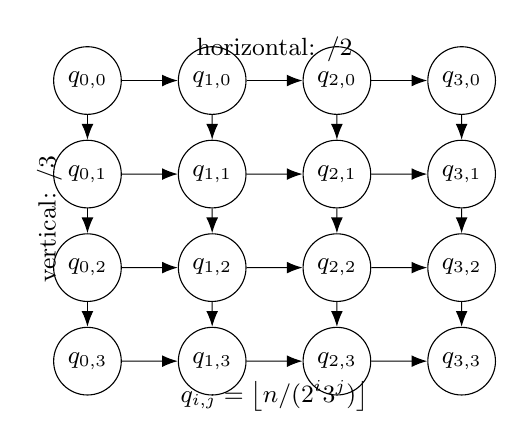
\begin{tikzpicture}[scale=0.88, every node/.style={font=\small}]
\foreach \i in {0,...,3}{
  \foreach \j in {0,...,3}{
    \node[circle,draw,minimum size=8mm] (q\i-\j) at (1.8*\i,-1.35*\j) {$q_{\i,\j}$};
  }
}
\draw[-{Latex[length=2mm]}] (q0-0)--(q1-0); \draw[-{Latex[length=2mm]}] (q1-0)--(q2-0); \draw[-{Latex[length=2mm]}] (q2-0)--(q3-0);
\draw[-{Latex[length=2mm]}] (q0-1)--(q1-1); \draw[-{Latex[length=2mm]}] (q1-1)--(q2-1); \draw[-{Latex[length=2mm]}] (q2-1)--(q3-1);
\draw[-{Latex[length=2mm]}] (q0-2)--(q1-2); \draw[-{Latex[length=2mm]}] (q1-2)--(q2-2); \draw[-{Latex[length=2mm]}] (q2-2)--(q3-2);
\draw[-{Latex[length=2mm]}] (q0-3)--(q1-3); \draw[-{Latex[length=2mm]}] (q1-3)--(q2-3); \draw[-{Latex[length=2mm]}] (q2-3)--(q3-3);
\draw[-{Latex[length=2mm]}] (q0-0)--(q0-1); \draw[-{Latex[length=2mm]}] (q0-1)--(q0-2); \draw[-{Latex[length=2mm]}] (q0-2)--(q0-3);
\draw[-{Latex[length=2mm]}] (q1-0)--(q1-1); \draw[-{Latex[length=2mm]}] (q1-1)--(q1-2); \draw[-{Latex[length=2mm]}] (q1-2)--(q1-3);
\draw[-{Latex[length=2mm]}] (q2-0)--(q2-1); \draw[-{Latex[length=2mm]}] (q2-1)--(q2-2); \draw[-{Latex[length=2mm]}] (q2-2)--(q2-3);
\draw[-{Latex[length=2mm]}] (q3-0)--(q3-1); \draw[-{Latex[length=2mm]}] (q3-1)--(q3-2); \draw[-{Latex[length=2mm]}] (q3-2)--(q3-3);
\node at (2.7,0.45) {horizontal: $/2$};
\node[rotate=90] at (-0.55,-2.0) {vertical: $/3$};
\node at (2.7,-4.55) {$q_{i,j}=\left\lfloor n/(2^i3^j)\right\rfloor$};
\end{tikzpicture}
\caption{The quotient lattice in the multiplicatively independent binary--ternary case. Different division words can merge at the same quotient state.}
\label{fig:lattice}
\end{figure}

\section{Maximal multipliers and defect monotonicity}
\begin{proposition}[Maximal multiplier]\label{prop:max}
If $M=\max D$, then
\[
 C_D(M^m)=m\qquad(m\ge0).
\]
\end{proposition}
\begin{proof}
The construction by $m$ multiplications by $M$ gives the upper bound. No unit-cost operation can increase a positive state by a factor exceeding $M$, so fewer than $m$ operations cannot reach $M^m$.
\end{proof}

For $d\in D$ define
\[
 \delta_{D,d}(m)=m-C_D(d^m).
\]
\begin{proposition}[Defect monotonicity]\label{prop:defectmono}
For every $d\in D$, $\delta_{D,d}(m)$ is nondecreasing in $m$.
\end{proposition}
\begin{proof}
Append one multiplication by $d$ to an optimal construction of $d^m$:
\[
 C_D(d^{m+1})\le C_D(d^m)+1.
\]
Rearrangement gives the claim.
\end{proof}
By Proposition~\ref{prop:max}, the maximal multiplier has identically zero defect.

\section{The first shortcut to a power of two}\label{sec:shortcut}
From here let $D=\{2,3\}$ and write $C=C_D$.

\begin{theorem}[First power-of-two shortcut]\label{thm:54}
\[
 C(2^m)=m\quad(1\le m\le53),
\qquad
 C(2^{54})=53.
\]
Among canonical normalized 53-step constructions of $2^{54}$, the unique operation-count signature is
\[
 \boxed{(a,b,c)=(8,29,16)}.
\]
\end{theorem}
The theorem is computer-assisted. The exact recurrence is evaluated directly at the relevant powers. Its implementation is cross-validated against an independently formulated forward $O(N)$ dynamic program for every $n\le10^6$. A separate fixed-count dynamic program recovers the target value and the unique canonical signature. All arithmetic is exact, and an explicit 53-operation primitive witness is supplied with the archival package.

\subsection{An exact signature identity}
The next theorem explains why operation counts are highly constrained.

\begin{lemma}[Canonical product envelope]\label{lem:envelope}
For a canonical binary--ternary construction
\[
 x_i=d_i x_{i-1}+r_i,
\quad d_i\in\{2,3\},\quad0\le r_i<d_i,
\quad x_0=1,
\]
let $P_i=\prod_{j\le i}d_j$. Then
\[
 \boxed{P_i\le x_i\le2P_i-1.}
\]
\end{lemma}
\begin{proof}
Induct on $i$. The lower bound is immediate from $r_i\ge0$. If $x_{i-1}\le2P_{i-1}-1$, then
\[
 x_i\le d_i(2P_{i-1}-1)+(d_i-1)=2P_i-1.
\]
\end{proof}

\begin{theorem}[Exact defect identity]\label{thm:defectidentity}
Suppose a canonical normalized construction of $2^m$ uses $a$ doublings, $b>0$ triplings, and $c$ increments. Put
\[
 \beta=\log_2(3/2).
\]
Then
\[
 \boxed{a=m-\lceil b\log_2 3\rceil}
\]
and its saving relative to $m$ pure doublings is exactly
\[
 \boxed{s=m-(a+b+c)=\lceil\beta b\rceil-c.}
\]
\end{theorem}
\begin{proof}
By Lemma~\ref{lem:envelope}, with $P=2^a3^b$,
\[
 P\le2^m<2P.
\]
Thus
\[
 m-1<a+b\log_2 3\le m.
\]
Because $b>0$, $b\log_2 3$ is irrational, so the integer $a$ is uniquely
\[
 a=m-\lceil b\log_2 3\rceil.
\]
Substituting into $s=m-a-b-c$ and using $\lceil b\log_2 3\rceil-b=\lceil b\log_2(3/2)\rceil$ proves the second identity.
\end{proof}

For $b=29$,
\[
 \lceil29\log_2(3/2)\rceil=17.
\]
Thus a one-step shortcut requires exactly $c=16$ increments. Moreover
\[
 \frac{3^{29}}{2^{46}}\approx0.9752963218,
\]
so 29 triplings provide almost the growth of 46 doublings: the nominal 17-operation multiplication saving is reduced by 16 unit corrections, leaving one net step.

\subsection{A 3-adic reason that 54 is exceptional}
\begin{proposition}[Four-tripling runway]\label{prop:runway}
For even $m$,
\[
 v_3(2^m-1)=1+v_3(m).
\]
Hence $m=54$ is the smallest positive even exponent for which $3^4\mid2^m-1$.
\end{proposition}
\begin{proof}
Write $2^m-1=4^{m/2}-1$. The lifting-the-exponent lemma gives
\[
 v_3(4^{m/2}-1)=v_3(4-1)+v_3(m/2)=1+v_3(m).
\]
The inequality $v_3(2^m-1)\ge4$ is equivalent to $27\mid m$; the smallest positive even such $m$ is $54$.
\end{proof}
Thus at $m=54$, a single initial reverse subtraction buys four consecutive exact divisions by $3$. A block of one subtraction and $k$ triplings has binary logarithmic gain
\[
 G_k=k\log_2 3-(k+1).
\]
Here $G_3<1$ while $G_4>1$. This isolates an arithmetic mechanism that first becomes available at exponent $54$; the exact proof that no globally different shortcut occurs earlier remains the finite exact computation of Theorem~\ref{thm:54}, not this local argument alone.

\section{Mersenne reduction of the power-of-two defect}
Define
\[
 \delta(m)=m-C(2^m).
\]
\begin{theorem}[Mersenne reduction]\label{thm:mersenne}
For every $m\ge1$,
\[
 \boxed{
 C(2^m)=\min\left\{m,\ \min_{1\le k\le m}\bigl[C(2^k-1)+1+m-k\bigr]\right\}.}
\]
Consequently
\[
 \boxed{
 \delta(m)=\max\left\{0,\ \max_{1\le k\le m}\bigl[k-1-C(2^k-1)\bigr]\right\}.}
\]
\end{theorem}
\begin{proof}
Take any construction of $2^m$ that uses an increment, and consider its last $+1$. After that operation only multiplications remain. No later multiplication can be by $3$, because the final result is a power of $2$. Hence the suffix consists of $m-k$ doublings for some $k$, and immediately after the last increment the state is $2^k$; immediately before it the state is $2^k-1$. Thus the prefix costs at least $C(2^k-1)$ and the whole program at least $C(2^k-1)+1+m-k$. Conversely each such prefix followed by $+1$ and $m-k$ doublings is a valid construction. Include the pure-doubling option $m$ and rearrange.
\end{proof}

This gives an exact equivalence:
\[
 \boxed{\sup_m\delta(m)=\infty\quad\Longleftrightarrow\quad
 \sup_k\bigl(k-1-C(2^k-1)\bigr)=\infty.}
\]
The power-of-two defect is therefore the running maximum of a Mersenne construction-saving sequence.

\section{Fixed-tripling profiles and a finite stopping theorem}
For $b\ge1$ define
\[
 k_b=\lceil b\log_2 3\rceil,
 \qquad d_b=k_b-b=\lceil b\log_2(3/2)\rceil.
\]
Let $c_b(a)$ be the minimum number of increments among canonical normalized constructions of
\[
 2^{a+k_b}
\]
using exactly $a$ doublings and $b$ triplings.

Residue normalization guarantees that every optimum has a canonical normalized reverse path. Therefore partitioning paths by the exact division counts $(a,b)$ covers every possible optimal operation-count signature; no unrestricted optimum is lost in the fixed-count profile.

\begin{proposition}[Stabilization]\label{prop:stabilization}
For fixed $b$, $c_b(a)$ is nonincreasing in $a$ and therefore eventually constant. Let its stable value be $c_b^\infty$. Then
\[
 \boxed{\sup_m\delta(m)=\sup_{b\ge1}\bigl(d_b-c_b^\infty\bigr).}
\]
\end{proposition}
\begin{proof}
Appending one final doubling to a construction counted by $c_b(a)$ gives a construction counted by $c_b(a+1)$ with the same number of increments, so $c_b(a+1)\le c_b(a)$. A nonincreasing sequence of nonnegative integers stabilizes. By Theorem~\ref{thm:defectidentity}, every canonical program with $b$ triplings has defect $d_b-c$, and every power-of-two optimum is represented in some fixed-count profile. Taking suprema gives the formula.
\end{proof}

The fixed-count recurrence used computationally is as follows. Let $R(n;a,b)$ be the minimum number of subtractions in a normalized reverse path from $n$ using exactly $a$ divisions by $2$ and $b$ divisions by $3$, after which the remaining state is reduced to $1$ by subtractions only. Set
\[
 R(n;0,0)=n-1.
\]
For $a+b>0$, infeasible states have value $+\infty$, and
\[
 R(n;a,b)=\min\begin{cases}
 (n\bmod2)+R(\lfloor n/2\rfloor;a-1,b),&a>0,\ n\ge2,\\
 (n\bmod3)+R(\lfloor n/3\rfloor;a,b-1),&b>0,\ n\ge3.
 \end{cases}
\]
Unavailable branches are omitted.

\begin{theorem}[Finite stopping bound]\label{thm:stopping}
Fix $b\ge1$. Suppose a correction level at most $c$ first occurs at $a=a_0>0$, i.e. $c_b(a_0)\le c$ but $c_b(a)>c$ for $a<a_0$. Then
\[
 \boxed{
 a_0\le \lceil b\log_2 3\rceil c+
 \sum_{j=1}^{b}\bigl(\lceil j\log_2 3\rceil-1\bigr).}
\]
Consequently, for every fixed $b$ and target correction level $c$, whether that level ever occurs is decidable by a finite search.
\end{theorem}
\begin{proof}
At the first occurrence $a_0$, an optimal reverse path cannot begin with the free division $2^{a_0+k_b}\mapsto2^{a_0+k_b-1}$; deleting it would realize the same correction level at $a_0-1$. Hence every binary division occurs after at least one ternary division.

At ternary level $j\ge1$, every state encountered between ternary divisions has the form
\[
 q=\left\lfloor\frac{2^t}{3^j}\right\rfloor.
\]
If $2^h\mid q$, write $2^t=3^jq+r$ with $0<r<3^j$. Then $2^h\mid r$, so
\[
 2^h<3^j,
\qquad
 h\le\lceil j\log_2 3\rceil-1.
\]
Thus each run of free binary divisions at level $j$ has length at most $L_j-1$, where $L_j=\lceil j\log_2 3\rceil$. If $p_j$ paid binary divisions occur at that level, there are at most $p_j+1$ free runs, so the total binary divisions there are at most
\[
 p_j+(p_j+1)(L_j-1)=L_jp_j+L_j-1.
\]
Every paid binary division costs at least one subtraction, hence $\sum_jp_j\le c$. Summing and using $L_j\le L_b$ gives
\[
 a_0\le L_b c+\sum_{j=1}^b(L_j-1).
\]
\end{proof}

The theorem converts each fixed-$b$ stabilization assertion from an infinite claim into a finite verification problem. It does \emph{not} by itself settle whether the stable defects $d_b-c_b^\infty$ are globally bounded as $b\to\infty$.

\section{Cheaper multiplicative relations in general multiplier sets}
The hard binary--ternary case is multiplicatively independent. In the dependent regime one can prove much more.

\begin{theorem}[Linear defect from a cheaper relation]\label{thm:relation}
Let $q\in D$. Suppose there is an exact relation
\[
 q^p=\prod_{e\in D}e^{r_e},
\qquad r_e\in\mathbb Z_{\ge0},
\]
with
\[
 R:=\sum_{e\in D}r_e<p.
\]
Then
\[
 \boxed{
 \delta_{D,q}(m)\ge(p-R)\left\lfloor\frac mp\right\rfloor,}
\]
so the defect of powers of $q$ is linearly unbounded.
\end{theorem}
\begin{proof}
Write $m=pt+s$, $0\le s<p$. Repeat the cheaper multiplicative representation of $q^p$ exactly $t$ times and then multiply by $q$ another $s$ times. This constructs $q^m$ in at most $Rt+s$ operations. Therefore
\[
 m-C_D(q^m)\ge pt+s-(Rt+s)=(p-R)t.
\]
\end{proof}

Together with Proposition~\ref{prop:max}, this separates two easy regimes: the maximal multiplier has zero defect forever, while any multiplier with a cheaper exact multiplicative relation has linear defect. The genuinely difficult regime consists of nonmaximal multipliers that are multiplicatively independent of the larger available multipliers, such as $2$ in $\{2,3\}$.

\section{Local swap law and the remaining algorithmic barrier}
Fix a reverse state $q$ and compare two adjacent orders, $/2$ then $/3$ versus $/3$ then $/2$. Both end at $\lfloor q/6\rfloor$. Their difference in subtraction cost is
\[
 \kappa(q)=(q\bmod2)+(\lfloor q/2\rfloor\bmod3)
 -(q\bmod3)-(\lfloor q/3\rfloor\bmod2).
\]
\begin{proposition}[Local swap law]\label{prop:swap}
\[
 \boxed{
 \kappa(q)=\begin{cases}
 -1,&q\equiv2\pmod6,\\
 +1,&q\equiv3\pmod6,\\
 0,&q\equiv0,1,4,5\pmod6.
 \end{cases}}
\]
\end{proposition}
\begin{proof}
Check the six residues modulo $6$.
\end{proof}

For fixed counts $(a,b)$, division words are monotone paths on the quotient grid
\[
 q_{i,j}=\left\lfloor\frac{n}{2^i3^j}\right\rfloor.
\]
Adjacent path swaps change cost by the local cell weight $\kappa(q_{i,j})\in\{-1,0,1\}$. Thus fixed-count optimization is a minimum-weight monotone-boundary problem on a highly structured arithmetic grid.

A purely local greedy rule is insufficient. For $n=15$ with two $/2$ divisions and one $/3$, the word $/2,/2,/3$ has correction cost $2$ and has no strictly improving immediate swap at its relevant tied cell, while $/3,/2,/2$ has correction cost $1$. Any exact $O(\log n)$ algorithm, if one exists, must exploit global arithmetic structure rather than local swaps alone.

A rolling-row implementation of the fixed-count grid uses $O((\log n)^2)$ arithmetic time and $O(\log n)$ memory for $D=\{2,3\}$. Whether the exact scalar problem admits $O(\log n)$ time remains open.

\section{Computational certification and reproducibility}
The reproducibility bundle prepared for deposit alongside this preprint contains \texttt{verify.py}, which uses exact Python integers only. It performs the following checks:
\begin{enumerate}
\item compares the compressed recurrence against an independently formulated forward $O(N)$ dynamic program for every $n\le10^6$;
\item verifies $C(2^m)=m$ for $1\le m\le53$ and $C(2^{54})=53$;
\item verifies that the unique canonical normalized 53-step signature at $2^{54}$ is $(8,29,16)$;
\item expands a 53-operation primitive certificate and checks every intermediate integer;
\item reproduces the first defect records through $m=1600$:
\[
 (54,1),\ (126,2),\ (1008,3),\ (1028,4);
\]
\item verifies the Mersenne reduction identity through $m=300$ as an implementation consistency check;
\item reproduces selected fixed-count profiles underlying the first four defect records;
\item verifies the local swap table and the $3$-adic runway at $m=54$.
\end{enumerate}

The forward DP is an independent finite-range implementation cross-check, not a direct second evaluation of $2^{54}$. At the headline target, the scalar recurrence is additionally checked by the separately formulated fixed-count profile computation and by the explicit primitive witness.

\begin{table}[t]
\centering
\caption{Selected exact fixed-count profiles.}
\begin{tabular}{rrrrrr}
\toprule
$m$ & $a$ & $b$ & $c$ & total & defect\\
\midrule
54&8&29&16&53&1\\
126&18&68&38&124&2\\
966&183&494&288&965&1\\
996&213&494&287&994&2\\
1008&225&494&286&1005&3\\
1028&245&494&285&1024&4\\
\bottomrule
\end{tabular}
\end{table}

The source distribution prepared for the Zenodo deposit contains the full source code, output logs, CSV tables, primitive certificate, and SHA-256 checksums. Until that Zenodo record is actually published, no archival DOI or public availability through the DOI is claimed. The DOI field remains \texttt{\ZenodoDOI}; the reserved DOI should be inserted into the manuscript only after a Zenodo draft has been created and before the record is published.

\section{Open problems}
These reductions isolate the remaining central questions.

\begin{question}[Power-of-two defect]
Is $\delta(m)=m-C(2^m)$ bounded or unbounded? Equivalently, by Theorem~\ref{thm:mersenne} and Proposition~\ref{prop:stabilization}, determine whether
\[
 \sup_k\bigl(k-1-C(2^k-1)\bigr)
 =
 \sup_{b\ge1}\bigl(\lceil b\log_2(3/2)\rceil-c_b^\infty\bigr)
\]
is finite.
\end{question}

\begin{question}[Asymptotics of stable correction]
Determine the asymptotic behavior of
\[
 \lceil b\log_2(3/2)\rceil-c_b^\infty.
\]
The finite stopping theorem makes every fixed-$b$ instance decidable, but gives no uniform asymptotic bound in $b$.
\end{question}

\begin{question}[Analytic threshold]
Can the exact threshold $m=54$ be derived without finite exhaustive evaluation? Proposition~\ref{prop:runway} explains why a four-tripling $3$-adic runway first appears at $54$, while Theorem~\ref{thm:defectidentity} forces the successful count balance, but a purely analytic exclusion of every competing $m\le53$ remains open.
\end{question}

\begin{question}[Linear-time exact algorithm]
Can $C(n)$ be computed in $O(\log n)$ arithmetic time, or can one prove a lower bound ruling this out in a natural computational model? Proposition~\ref{prop:swap} shows that simple local swap optimization is insufficient.
\end{question}

\begin{question}[Independent nonmaximal multipliers]
For general $D$, characterize the defect of a nonmaximal multiplier that is multiplicatively independent of the larger multipliers. Theorem~\ref{thm:relation} settles the cheaper-relation regime, while Proposition~\ref{prop:max} settles the maximal multiplier.
\end{question}

\section{Conclusion}
A shortest-path problem with three elementary unary operations hides a rigid arithmetic structure. Residue normalization turns the unrestricted problem into an exact mixed-radix system; multiplicative rank controls the quotient-state geometry; smooth-minus-one inputs satisfy a boundary law; and powers of two admit an exact defect identity and Mersenne reduction. The first shortcut at $2^{54}$ is therefore not an isolated computational curiosity but the first visible point of a broader defect theory. The central unresolved problem is now precise: understand the stable correction deficit
\[
 \lceil b\log_2(3/2)\rceil-c_b^\infty.
\]

\section*{Data and code availability}
The manuscript source, exact verifier, generated certificates and tables, metadata, and checksums are included in the reproducibility bundle prepared for deposit with this preprint. At the time of this version, the Zenodo record has not yet been published and no public DOI is claimed. Zenodo DOI: \texttt{\ZenodoDOI} (to be reserved in the deposit draft and inserted before publication).

\section*{Acknowledgments}
The author thanks the maintainers of the OEIS and the authors of the cited mixed-radix, multi-base, and integer-complexity literature for providing useful context for this problem.

\begin{thebibliography}{99}
\bibitem{OEIS}
N. J. A. Sloane et al., \emph{The On-Line Encyclopedia of Integer Sequences}, A056796, minimum number of steps from $0$ to $n$ using increment, doubling, and tripling. For the normalization used here, $a(n)=C(n)+1$ for $n\ge1$. \url{https://oeis.org/A056796}.

\bibitem{Amano2022}
K. Amano, ``Integer Complexity and Mixed Binary-Ternary Representation,'' \emph{LIPIcs ISAAC 2022}, vol. 248, Article 29, 2022. DOI: \href{https://doi.org/10.4230/LIPIcs.ISAAC.2022.29}{10.4230/LIPIcs.ISAAC.2022.29}.

\bibitem{KrennSuppakitpaisarnWagner2020}
D. Krenn, V. Suppakitpaisarn, and S. Wagner, ``On the minimal Hamming weight of a multi-base representation,'' \emph{Journal of Number Theory} 208 (2020), 168--179. Preprint: \url{https://arxiv.org/abs/1808.06330}.

\bibitem{DimitrovHowe2010}
V. S. Dimitrov and E. W. Howe, ``Lower bounds on the lengths of double-base representations,'' arXiv:1001.4133, 2010. \url{https://arxiv.org/abs/1001.4133}.

\bibitem{Simon2025}
D. Simon, ``Mixed radix numeration bases: Horner's rule, Yang--Baxter equation and Furstenberg's conjecture,'' \emph{Combinatorial Theory} 5(2), 2025. DOI: \href{https://doi.org/10.5070/C65265419}{10.5070/C65265419}.

\bibitem{BernsteinChuengsatiansupLange2017}
D. J. Bernstein, S. Chuengsatiansup, and T. Lange, ``Double-base scalar multiplication revisited,'' Cryptology ePrint Archive, Report 2017/037, 2017. \url{https://eprint.iacr.org/2017/037}.

\bibitem{Lagarias2009}
J. C. Lagarias, ``Ternary expansions of powers of 2,'' \emph{Journal of the London Mathematical Society} 79(3) (2009), 562--588. DOI: \href{https://doi.org/10.1112/jlms/jdn080}{10.1112/jlms/jdn080}.

\bibitem{CernenoksEtAl2014}
J. \v{C}er\c{n}enoks, J. Iraids, M. Opmanis, R. Opmanis, and K. Podnieks, ``Integer Complexity: Experimental and Analytical Results II,'' arXiv:1409.0446, 2014. \url{https://arxiv.org/abs/1409.0446}.

\bibitem{Bahig2008}
H. M. Bahig, ``On a generalization of addition chains: Addition--multiplication chains,'' \emph{Discrete Mathematics} 308(4) (2008), 611--616. DOI: \href{https://doi.org/10.1016/j.disc.2007.04.015}{10.1016/j.disc.2007.04.015}.

\bibitem{TarekBahigAnwar2026}
M. Tarek, H. M. Bahig, and N. Anwar, ``Addition-multiplication chains with one small step,'' \emph{AIMS Mathematics} 11(6) (2026), 16235--16263. DOI: \href{https://doi.org/10.3934/Math.2026667}{10.3934/Math.2026667}.
\end{thebibliography}

\end{document}
